
%% bare_jrnl_transmag.tex
%% V1.4a
%% 2014/09/17
%% by Michael Shell
%% see http://www.michaelshell.org/
%% for current contact information.
%%
%% This is a skeleton file demonstrating the use of IEEEtran.cls
%% (requires IEEEtran.cls version 1.8a or later) with an IEEE 
%% Transactions on Magnetics journal paper.
%%
%% Support sites:
%% http://www.michaelshell.org/tex/ieeetran/
%% http://www.ctan.org/tex-archive/macros/latex/contrib/IEEEtran/
%% and
%% http://www.ieee.org/

%%*************************************************************************
%% Legal Notice:
%% This code is offered as-is without any warranty either expressed or
%% implied; without even the implied warranty of MERCHANTABILITY or
%% FITNESS FOR A PARTICULAR PURPOSE! 
%% User assumes all risk.
%% In no event shall IEEE or any contributor to this code be liable for
%% any damages or losses, including, but not limited to, incidental,
%% consequential, or any other damages, resulting from the use or misuse
%% of any information contained here.
%%
%% All comments are the opinions of their respective authors and are not
%% necessarily endorsed by the IEEE.
%%
%% This work is distributed under the LaTeX Project Public License (LPPL)
%% ( http://www.latex-project.org/ ) version 1.3, and may be freely used,
%% distributed and modified. A copy of the LPPL, version 1.3, is included
%% in the base LaTeX documentation of all distributions of LaTeX released
%% 2003/12/01 or later.
%% Retain all contribution notices and credits.
%% ** Modified files should be clearly indicated as such, including  **
%% ** renaming them and changing author support contact information. **
%%
%% File list of work: IEEEtran.cls, IEEEtran_HOWTO.pdf, bare_adv.tex,
%%                    bare_conf.tex, bare_jrnl.tex, bare_conf_compsoc.tex,
%%                    bare_jrnl_compsoc.tex, bare_jrnl_transmag.tex
%%*************************************************************************


% *** Authors should verify (and, if needed, correct) their LaTeX system  ***
% *** with the testflow diagnostic prior to trusting their LaTeX platform ***
% *** with production work. IEEE's font choices and paper sizes can       ***
% *** trigger bugs that do not appear when using other class files.       ***                          ***
% The testflow support page is at:
% http://www.michaelshell.org/tex/testflow/



\documentclass[journal,transmag,twoside]{IEEEtran}
%
% If IEEEtran.cls has not been installed into the LaTeX system files,
% manually specify the path to it like:
% \documentclass[journal]{../sty/IEEEtran}





% Some very useful LaTeX packages include:
% (uncomment the ones you want to load)


% *** MISC UTILITY PACKAGES ***
%
%\usepackage{ifpdf}
% Heiko Oberdiek's ifpdf.sty is very useful if you need conditional
% compilation based on whether the output is pdf or dvi.
% usage:
% \ifpdf
%   % pdf code
% \else
%   % dvi code
% \fi
% The latest version of ifpdf.sty can be obtained from:
% http://www.ctan.org/tex-archive/macros/latex/contrib/oberdiek/
% Also, note that IEEEtran.cls V1.7 and later provides a builtin
% \ifCLASSINFOpdf conditional that works the same way.
% When switching from latex to pdflatex and vice-versa, the compiler may
% have to be run twice to clear warning/error messages.






% *** CITATION PACKAGES ***
%
%\usepackage{cite}
% cite.sty was written by Donald Arseneau
% V1.6 and later of IEEEtran pre-defines the format of the cite.sty package
% \cite{} output to follow that of IEEE. Loading the cite package will
% result in citation numbers being automatically sorted and properly
% "compressed/ranged". e.g., [1], [9], [2], [7], [5], [6] without using
% cite.sty will become [1], [2], [5]--[7], [9] using cite.sty. cite.sty's
% \cite will automatically add leading space, if needed. Use cite.sty's
% noadjust option (cite.sty V3.8 and later) if you want to turn this off
% such as if a citation ever needs to be enclosed in parenthesis.
% cite.sty is already installed on most LaTeX systems. Be sure and use
% version 5.0 (2009-03-20) and later if using hyperref.sty.
% The latest version can be obtained at:
% http://www.ctan.org/tex-archive/macros/latex/contrib/cite/
% The documentation is contained in the cite.sty file itself.






% *** GRAPHICS RELATED PACKAGES ***
%
\ifCLASSINFOpdf
  \usepackage[pdftex]{graphicx}
  % declare the path(s) where your graphic files are
  % \graphicspath{{../pdf/}{../jpeg/}}
  % and their extensions so you won't have to specify these with
  % every instance of \includegraphics
  % \DeclareGraphicsExtensions{.pdf,.jpeg,.png}
\else
  % or other class option (dvipsone, dvipdf, if not using dvips). graphicx
  % will default to the driver specified in the system graphics.cfg if no
  % driver is specified.
  % \usepackage[dvips]{graphicx}
  % declare the path(s) where your graphic files are
  % \graphicspath{{../eps/}}
  % and their extensions so you won't have to specify these with
  % every instance of \includegraphics
  % \DeclareGraphicsExtensions{.eps}
\fi
% graphicx was written by David Carlisle and Sebastian Rahtz. It is
% required if you want graphics, photos, etc. graphicx.sty is already
% installed on most LaTeX systems. The latest version and documentation
% can be obtained at: 
% http://www.ctan.org/tex-archive/macros/latex/required/graphics/
% Another good source of documentation is "Using Imported Graphics in
% LaTeX2e" by Keith Reckdahl which can be found at:
% http://www.ctan.org/tex-archive/info/epslatex/
%
% latex, and pdflatex in dvi mode, support graphics in encapsulated
% postscript (.eps) format. pdflatex in pdf mode supports graphics
% in .pdf, .jpeg, .png and .mps (metapost) formats. Users should ensure
% that all non-photo figures use a vector format (.eps, .pdf, .mps) and
% not a bitmapped formats (.jpeg, .png). IEEE frowns on bitmapped formats
% which can result in "jaggedy"/blurry rendering of lines and letters as
% well as large increases in file sizes.
%
% You can find documentation about the pdfTeX application at:
% http://www.tug.org/applications/pdftex




% *** MATH PACKAGES ***
%
%\usepackage[cmex10]{amsmath}
% A popular package from the American Mathematical Society that provides
% many useful and powerful commands for dealing with mathematics. If using
% it, be sure to load this package with the cmex10 option to ensure that
% only type 1 fonts will utilized at all point sizes. Without this option,
% it is possible that some math symbols, particularly those within
% footnotes, will be rendered in bitmap form which will result in a
% document that can not be IEEE Xplore compliant!
%
% Also, note that the amsmath package sets \interdisplaylinepenalty to 10000
% thus preventing page breaks from occurring within multiline equations. Use:
%\interdisplaylinepenalty=2500
% after loading amsmath to restore such page breaks as IEEEtran.cls normally
% does. amsmath.sty is already installed on most LaTeX systems. The latest
% version and documentation can be obtained at:
% http://www.ctan.org/tex-archive/macros/latex/required/amslatex/math/





% *** SPECIALIZED LIST PACKAGES ***
%
%\usepackage{algorithmic}
% algorithmic.sty was written by Peter Williams and Rogerio Brito.
% This package provides an algorithmic environment fo describing algorithms.
% You can use the algorithmic environment in-text or within a figure
% environment to provide for a floating algorithm. Do NOT use the algorithm
% floating environment provided by algorithm.sty (by the same authors) or
% algorithm2e.sty (by Christophe Fiorio) as IEEE does not use dedicated
% algorithm float types and packages that provide these will not provide
% correct IEEE style captions. The latest version and documentation of
% algorithmic.sty can be obtained at:
% http://www.ctan.org/tex-archive/macros/latex/contrib/algorithms/
% There is also a support site at:
% http://algorithms.berlios.de/index.html
% Also of interest may be the (relatively newer and more customizable)
% algorithmicx.sty package by Szasz Janos:
% http://www.ctan.org/tex-archive/macros/latex/contrib/algorithmicx/




% *** ALIGNMENT PACKAGES ***
%
%\usepackage{array}
% Frank Mittelbach's and David Carlisle's array.sty patches and improves
% the standard LaTeX2e array and tabular environments to provide better
% appearance and additional user controls. As the default LaTeX2e table
% generation code is lacking to the point of almost being broken with
% respect to the quality of the end results, all users are strongly
% advised to use an enhanced (at the very least that provided by array.sty)
% set of table tools. array.sty is already installed on most systems. The
% latest version and documentation can be obtained at:
% http://www.ctan.org/tex-archive/macros/latex/required/tools/


% IEEEtran contains the IEEEeqnarray family of commands that can be used to
% generate multiline equations as well as matrices, tables, etc., of high
% quality.




% *** SUBFIGURE PACKAGES ***
%\ifCLASSOPTIONcompsoc
%  \usepackage[caption=false,font=normalsize,labelfont=sf,textfont=sf]{subfig}
%\else
%  \usepackage[caption=false,font=footnotesize]{subfig}
%\fi
% subfig.sty, written by Steven Douglas Cochran, is the modern replacement
% for subfigure.sty, the latter of which is no longer maintained and is
% incompatible with some LaTeX packages including fixltx2e. However,
% subfig.sty requires and automatically loads Axel Sommerfeldt's caption.sty
% which will override IEEEtran.cls' handling of captions and this will result
% in non-IEEE style figure/table captions. To prevent this problem, be sure
% and invoke subfig.sty's "caption=false" package option (available since
% subfig.sty version 1.3, 2005/06/28) as this is will preserve IEEEtran.cls
% handling of captions.
% Note that the Computer Society format requires a larger sans serif font
% than the serif footnote size font used in traditional IEEE formatting
% and thus the need to invoke different subfig.sty package options depending
% on whether compsoc mode has been enabled.
%
% The latest version and documentation of subfig.sty can be obtained at:
% http://www.ctan.org/tex-archive/macros/latex/contrib/subfig/



% *** FLOAT PACKAGES ***
%
%\usepackage{fixltx2e}
% fixltx2e, the successor to the earlier fix2col.sty, was written by
% Frank Mittelbach and David Carlisle. This package corrects a few problems
% in the LaTeX2e kernel, the most notable of which is that in current
% LaTeX2e releases, the ordering of single and double column floats is not
% guaranteed to be preserved. Thus, an unpatched LaTeX2e can allow a
% single column figure to be placed prior to an earlier double column
% figure. The latest version and documentation can be found at:
% http://www.ctan.org/tex-archive/macros/latex/base/


%\usepackage{stfloats}
% stfloats.sty was written by Sigitas Tolusis. This package gives LaTeX2e
% the ability to do double column floats at the bottom of the page as well
% as the top. (e.g., "\begin{figure*}[!b]" is not normally possible in
% LaTeX2e). It also provides a command:
%\fnbelowfloat
% to enable the placement of footnotes below bottom floats (the standard
% LaTeX2e kernel puts them above bottom floats). This is an invasive package
% which rewrites many portions of the LaTeX2e float routines. It may not work
% with other packages that modify the LaTeX2e float routines. The latest
% version and documentation can be obtained at:
% http://www.ctan.org/tex-archive/macros/latex/contrib/sttools/
% Do not use the stfloats baselinefloat ability as IEEE does not allow
% \baselineskip to stretch. Authors submitting work to the IEEE should note
% that IEEE rarely uses double column equations and that authors should try
% to avoid such use. Do not be tempted to use the cuted.sty or midfloat.sty
% packages (also by Sigitas Tolusis) as IEEE does not format its papers in
% such ways.
% Do not attempt to use stfloats with fixltx2e as they are incompatible.
% Instead, use Morten Hogholm'a dblfloatfix which combines the features
% of both fixltx2e and stfloats:
%
% \usepackage{dblfloatfix}
% The latest version can be found at:
% http://www.ctan.org/tex-archive/macros/latex/contrib/dblfloatfix/




%\ifCLASSOPTIONcaptionsoff
%  \usepackage[nomarkers]{endfloat}
% \let\MYoriglatexcaption\caption
% \renewcommand{\caption}[2][\relax]{\MYoriglatexcaption[#2]{#2}}
%\fi
% endfloat.sty was written by James Darrell McCauley, Jeff Goldberg and 
% Axel Sommerfeldt. This package may be useful when used in conjunction with 
% IEEEtran.cls'  captionsoff option. Some IEEE journals/societies require that
% submissions have lists of figures/tables at the end of the paper and that
% figures/tables without any captions are placed on a page by themselves at
% the end of the document. If needed, the draftcls IEEEtran class option or
% \CLASSINPUTbaselinestretch interface can be used to increase the line
% spacing as well. Be sure and use the nomarkers option of endfloat to
% prevent endfloat from "marking" where the figures would have been placed
% in the text. The two hack lines of code above are a slight modification of
% that suggested by in the endfloat docs (section 8.4.1) to ensure that
% the full captions always appear in the list of figures/tables - even if
% the user used the short optional argument of \caption[]{}.
% IEEE papers do not typically make use of \caption[]'s optional argument,
% so this should not be an issue. A similar trick can be used to disable
% captions of packages such as subfig.sty that lack options to turn off
% the subcaptions:
% For subfig.sty:
% \let\MYorigsubfloat\subfloat
% \renewcommand{\subfloat}[2][\relax]{\MYorigsubfloat[]{#2}}
% However, the above trick will not work if both optional arguments of
% the \subfloat command are used. Furthermore, there needs to be a
% description of each subfigure *somewhere* and endfloat does not add
% subfigure captions to its list of figures. Thus, the best approach is to
% avoid the use of subfigure captions (many IEEE journals avoid them anyway)
% and instead reference/explain all the subfigures within the main caption.
% The latest version of endfloat.sty and its documentation can obtained at:
% http://www.ctan.org/tex-archive/macros/latex/contrib/endfloat/
%
% The IEEEtran \ifCLASSOPTIONcaptionsoff conditional can also be used
% later in the document, say, to conditionally put the References on a 
% page by themselves.




% *** PDF, URL AND HYPERLINK PACKAGES ***
%
\usepackage{url}
% url.sty was written by Donald Arseneau. It provides better support for
% handling and breaking URLs. url.sty is already installed on most LaTeX
% systems. The latest version and documentation can be obtained at:
% http://www.ctan.org/tex-archive/macros/latex/contrib/url/
% Basically, \url{my_url_here}.

\usepackage{hyperref}
\newcommand{\email}[1]{\href{mailto:#1}{#1}}

\usepackage{pdfcomment}
\usepackage{xcolor}
\newcommand{\karrcomment}[2]{\pdfmarkupcomment[markup=Highlight,color=yellow,author={Jonathan Karr}]{#1}{#2}}


% *** Do not adjust lengths that control margins, column widths, etc. ***
% *** Do not use packages that alter fonts (such as pslatex).         ***
% There should be no need to do such things with IEEEtran.cls V1.6 and later.
% (Unless specifically asked to do so by the journal or conference you plan
% to submit to, of course. )

\usepackage{color,soul} % for highlighting only

%http://tex.stackexchange.com/questions/61265/why-doesnt-the-ieeetran-document-class-recognize-definition-environments
\newtheorem{definition}{Definition}

% correct bad hyphenation here
\hyphenation{op-tical net-works semi-conduc-tor}

% Nature News on irreproducibility:
% http://www.nature.com/news/reproducibility-1.17552

\begin{document}

\title{Engineering Dynamical Models for Better Reproducibility}

\author{
    J. Kyle Medley$^*$ and
	Jonathan R. Karr
    
    \thanks{
        Manuscript received XXX XX, 2015; revised XXX XX, 201X; accepted XXX XX, 201X. Date of publication XXX XX, 201X; date of current version XXX XX, 201X.
        J. K. Medley was supported by NIH grant R01 GM081070. J. R. Karr was supported by NSF grant 1548123 and a James S McDonnell Foundation Postdoctoral Fellowship Award in Studying Complex Systems. The content is solely the responsibility of the authors and does not necessarily represent the views of the National Institutes of Health or the James S. McDonnell Foundation.
        \textit{Asterisk indicates corresponding author.}
    }
    \thanks{$^*$J. K. Medley is with the Department of Bioengineering, University of Washington, Seattle, WA 98195, USA (e-mail: \email{medleyj@uw.edu}).}
    \thanks{J. R. Karr is with the Department of Genetics \& Genomic Sciences, Icahn School of Medicine at Mount Sinai, New York, NY 10029, USA (e-mail: \email{karr@mssm.edu}).}
    \thanks{Digital Object Identifier 10.1109/TBME.XXXX.XXXXXXX}
}

% The paper headers
\markboth{IEEE Transactions on Biomedical Engineering,~Vol.~13, No.~9, September~2015}%
{Medley \MakeLowercase{\textit{et al.}}: Enginnering Dynamical Models for Better Reproducibility}
% The only time the second header will appear is for the odd numbered pages
% after the title page when using the twoside option.
% 
% *** Note that you probably will NOT want to include the author's ***
% *** name in the headers of peer review papers.                   ***
% You can use \ifCLASSOPTIONpeerreview for conditional compilation here if
% you desire.




% If you want to put a publisher's ID mark on the page you can do it like
% this:
%\IEEEpubid{0000--0000/00\$00.00~\copyright~2014 IEEE}
% Remember, if you use this you must call \IEEEpubidadjcol in the second
% column for its text to clear the IEEEpubid mark.



% use for special paper notices
%\IEEEspecialpapernotice{(Invited Paper)}

\maketitle

\begin{abstract}
Dynamical modeling has made great strides with the creation of the first whole-cell model of \textit{Mycoplasma genitalium}.
Continuing to advance dynamical modeling requires reproducing increasingly complex models and simulations. 
However, it is currently challenging to reproduce complex simulations. Here, we outline the requirements for reproducible modeling
and describe the standards and software tools that are needed to enable researchers to reproduce models and simulations. 
We use whole-cell modeling an an example throughout our discussion.
\end{abstract}

\begin{IEEEkeywords}
Systems biology, computational modeling, reproducibility
\end{IEEEkeywords}

% To allow for easy dual compilation without having to reenter the
% abstract/keywords data, the \IEEEtitleabstractindextext text will
% not be used in maketitle, but will appear (i.e., to be "transported")
% here as \IEEEdisplaynontitleabstractindextext when the compsoc 
% or transmag modes are not selected <OR> if conference mode is selected 
% - because all conference papers position the abstract like regular
% papers do.
\IEEEdisplaynontitleabstractindextext
% \IEEEdisplaynontitleabstractindextext has no effect when using
% compsoc or transmag under a non-conference mode.







% For peer review papers, you can put extra information on the cover
% page as needed:
% \ifCLASSOPTIONpeerreview
% \begin{center} \bfseries EDICS Category: 3-BBND \end{center}
% \fi
%
% For peerreview papers, this IEEEtran command inserts a page break and
% creates the second title. It will be ignored for other modes.
\IEEEpeerreviewmaketitle



\section{Introduction}
% The very first letter is a 2 line initial drop letter followed
% by the rest of the first word in caps.
% 
% form to use if the first word consists of a single letter:
% \IEEEPARstart{A}{demo} file is ....
% 
% form to use if you need the single drop letter followed by
% normal text (unknown if ever used by IEEE):
% \IEEEPARstart{A}{}demo file is ....
% 
% Some journals put the first two words in caps:
% \IEEEPARstart{T}{his demo} file is ....
% 
% Here we have the typical use of a "T" for an initial drop letter
% and "HIS" in caps to complete the first word.
\IEEEPARstart{R}{eproducibility} is one of the central tenets of the scientific method.
\textit{Reproducibility} is the ability to confirm a result via a completely independent test, including different investigators, experimental methods, and experimental machinery. 
This rigorous standard eliminates conclusions that were based on incorrect methods, machinery, or experiments and ensures that scientific results are only accepted as facts once multiple scientists have thoroughly dismissed other potential explanations. 

\textit{Replicability}, in contrast, is the ability to reproduce a result given the same experimental machinery and conditions. 
Replicability is a more liberal standard than reproducibility because replicability does not require independent experimental methods or equipment.
Consequently, replicability only has the power to eliminate conclusions that were based on erroneous experiments, and cannot eliminate conclusions based on faulty methods or machinery.

Due to the complexity of modern scientific experiments and financial, time, and publishing pressures, investigators often do not have the time or resources to design orthogonal methods to test results independently. Instead, investigators frequently replicate reported results using the published method. The underemphasis on independent testing has the potential to allow us to accept false results based on faulty methods.

Computational biology has become more replicable over the past several years through the introduction of standards including CellML \cite{cuellar2003overview}, SBML \cite{hucka2003}, SED-ML \cite{sedml2011}, the COMBINE archive \cite{COMBINE2012}, and SBGN \cite{LeNovereHMMSS09} and model repositories including BioModels and CellML Model Repository. These standards and repositories have enabled researchers to easily replicate most \textit{in silico} experiments using the same mathematical model, the same simulator, and the same parameter values. These standards and repositories have also enabled researchers to reuse models for new experiments, to expand models, and to combine submodels into larger, more comprehensive models.

Unfortunately, due to continued time pressures, the priority for innovation, and the growing complexity of computational methods, this increased emphasis on replicability has not translated into increased reproducibility. This is exemplified by the recent \textit{Mycoplasma genitalium} whole-cell model \cite{Karr2012}. The authors took great strides to ensure that their software could replicate results given the same initial conditions and random number generator seed. However, the novelty and complexity of the model make it difficult for other researchers to reproduce the model or its scientific conclusions.

Waltemath and Schreiber recently organized a week-long workshop to reproduce the \textit{M. genitalium} model simulations using SBML and open-source modeling software. The workshop included 60 modelers, modeling software developers, and standards developers. The workshop made great progress toward reproducing the model simulations in SBML, including draft SBML versions of most of the submodels. However, because the model requires many new SBML languages features that are still only supported by a few software programs and because the model is large, significant work remains to reproduce the model despite the more than one person-year of effort that has already been dedicated to reproducing the model simulations.

Here, we outline the requirements for reproducibility, show how they can
be achieved in simulation standards and software, and discuss how this would benefit
the computational biology field. We also show how these principles apply to the \textit{Mycoplasma genitalium} whole-cell
model.
Finally, we discuss how the biological modeling community can work toward standards
and tools which enable better reproducibility of complex models.

\begin{figure*}[!t]
\centering
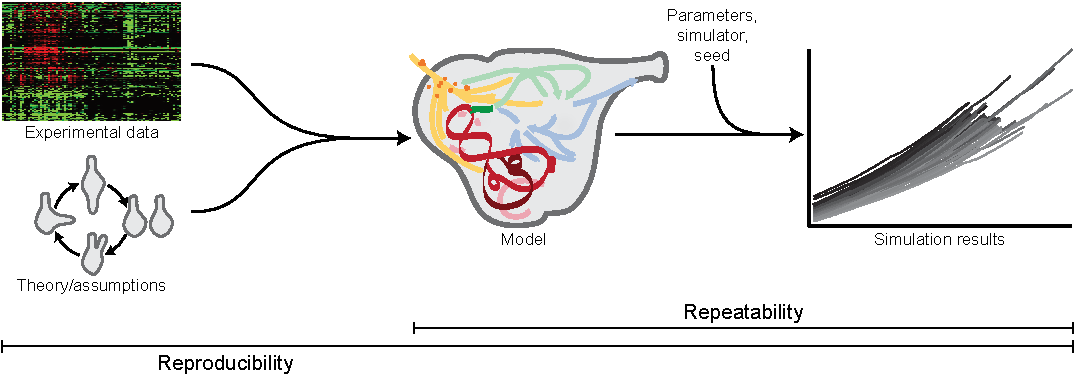
\includegraphics[width=\textwidth]{figure1/figure1}
% where an .eps filename suffix will be assumed under latex,
% and a .pdf suffix will be assumed for pdflatex; or what has been declared
% via \DeclareGraphicsExtensions.
\caption{Replicability and reproducibility explained: Model reproducibility refers to derivation from scientific knowledge and the ability to generate results in a reliable, repeatable manner;
Replicability refers only to the ability to recapitulate earlier simulation results}
\label{fig_repro_diagram}
\end{figure*}

\section{Replicability and Reproducibility}

In order to analyze which factors influence model reproducibility,
it is helpful to consider a subdomain of it: Replicability.
Replicability of a computational model refers to the ability to
re-run a simulation and obtain identical results \cite{easterbrook2014open}.

Variability in a model's output interferes with reproduction of the model.
If the model itself cannot converge on a solution, exact recapitulation of the model's behavior
becomes futile. %, and reproduction takes on a foggy meaning.
We do not address such cases in this paper, as the meaning of reproducibility in the face
of intrinsic variability becomes clouded.
Therefore, in order for a model to be reproducible, we require it to also be replicable,
as show in Fig. \ref{fig_repro_diagram}.

For a simulation result (such as a published figure) to meet our definition of replicability,
it must be possible to regenerate the result,
even if the simulation is run on a different machine.
Consequently, simulations can only be replicated if they are implemented using deterministic numerical solvers and
machine-independent pseudorandom processes.

A typical procedure for constructing a dynamical biological model
involves building and testing subsystems independently.
These tests, together with their coverage of known behavior of the system, provide a means to verify
that the model reproduces the experimentally verified functions of the biological system.
The tests can also serve as the foundation for independently reconstructing the model.
That is, model reproduction begins with reproducing each test in turn, and checking
the output of the new model against the original one.

If the test results cannot be replicated from run to run, the difficulty of reconstruction
increases dramatically, as results can no longer be directly compared but must instead
be compared using some metric of similarity.
The implication behind comparing stochastic models is that some summary of the data,
such as the mean and standard deviation, is sufficient to capture the behavior of the
model.
This is a difficult question to answer in general.
% Such a metric will by tacitly exclude features which are "random," and unimportant, and
% preserve others which are important and representative of the model dynamics.
Any behavioral discrepancy between the original model and its reconstruction
then has two possible causes: Algorithmic non-determinism or a deviation in dynamical
behavior.
% Sorting out how to compare two intrinsically variable models is case-dependent,
% as the features of interest are determined by the scientific questions the model is
% designed to address.
This imposes a burden on model reproduction, and can forestall or even prevent
model reconstruction efforts.
A software system engineered for model reproducibility should therefore possess
replicability as a first step.

Replicability, together with transparency, parameterization, documentation,
and annotation are essential for reproducible modeling.
These problems have been discussed within disparate contexts, but
have not been addressed in a unified way.
Recently, a division of labor has emerged which places software developers and
software users in separate spheres within the scientific community \cite{mesirov2010computer}.
Whereas technological solutions have been proposed to address replicability and reproducibility
of dynamical models \cite{bergmann2014combine} \cite{waltemath2011minimum} \cite{novere2005minimum},
a unified modeling platform supporting all of these features does not yet exist.
We envision such a platform would enable researchers to construct models in a
more open and standard way, and would cause use of these replicability and reproducibility
tools to become a standard practice among modelers.

Transparency is essential to achieving reproducibility for complex models \cite{boulton2012open}.
Making source code publicly available and freely reusable is an important step in this direction \cite{easterbrook2014open}.
However, a systematic framework for transparency is necessary to the continued success of whole-cell modeling.
The encoding of a model plays an important role in how easy it is to independently reproduce.
Using a standard representation which is widely understood makes a model more amenable to
independent scrutiny.
On top of this, another issue concerns how to preserve and encode the data used in the
model's construction.
The ideal goal should be record the source of all data used in a model in a machine-readable database .
The parameter values used in the \textit{M. genitalium} model are contained in an associated database, WholeCellKB-MG \cite{karr2013wholecellkb}.

Reproducing a model independently requires validating its assumptions,
which is not a topic addressed by current standards.
Given that many biochemical reactions are cataloged in databases such as
KEGG \cite{kanehisa2000kegg}, MetaCyc \cite{caspi2008metacyc}, BRENDA \cite{schomburg2002brenda}, and
ExplorEnz \cite{mcdonald2009explorenz}, there is clearly a potential for
linking SBML elements to the biophysical entities (e.g. molecules and reactions) they represent.
Relevant information, such as the biological underpinnings
of each dynamical processes, as well as the specific numerical values used by parameters,
could in principle be collected by model repositories such as BioModels \cite{le2006biomodels}
and linked to their respective sources.
This would both improve model credibility and allow others to efficiently
query, validate, and reconstruct a model from its assumptions,
an activity which is currently laborious due to the necessity of manual verification.

Whole-cell models make extensive use of experimentally measured single-cell parameters.
In the \textit{M. genitalium} model, much of this data comes from the literature.
Over 900 papers and 1,900 experimentally observed parameters were used to construct the model \cite{Karr2012}.
Many of the parameters of the model were based on measurements made in other species \cite{macklin2014future}.
As new measurements are made, more accurate models can be built.
However, this relies on continual improvement in experimental reliability.
One way to achieve this is to deposit experimental results into repositories
containing redundant data and associated meta-information including
a detailed record of experimental conditions and procedures.
In the model, the sources for various types of experimental data must be preserved,
as well as the rationale behind using them in a particular setting
(e.g. the choice of parameter values).
Future advances may help to automate this process, thus accelerating model development.

In summary, to be reproducible, a model must be replicable, and it must be encoded
in a transparent, reusable format. The data used in its construction must be
recorded in an easily accessible way.

\subsection{Limitations of Current Standards for Reproducibile Modeling}

The CellML \cite{cuellar2003overview}, SBML \cite{hucka2003}, and SED-ML \cite{sedml2011} standards have greatly improved the replicability of dynamical modeling.
Despite these advances, results in computational biology still cannot easily be reproduced \cite{garijo2013quantifying}.

Part of this difficulty can be attributed to gaps in standards.
SED-ML, for example, has good coverage of simulation parameters, but
does not address the determinism or lack thereof in the underlying simulator.
Whereas some modeling techniques such as ordinary differential equations (ODEs)
are typically highly replicable, other methods such as Gillespie's SSA and
and Markov processes are not. These methods are inherently stochastic and care
must be taken to ensure that they give identical results on different machines.
Replicability of inherently stochastic processes is not currently addressed by standards,
and each software tool must implement its own solution.

Other concerns, such as data transparency, play an important role that is becoming more apparent.
With the emergence of complex hybrid models, more researchers have noted the increased demand for curated, high quality measurements in order to improve the current state-of-the-art pathway and genome databases.

Another barrier to reproducibility concerns limited support for standards.
One advantage of representing a model in a standard format such as SBML is the ability
to utilize different simulators.
SBML Level 3 consists of extensions which enable additional
functionality, such as
hierarchical model composition\footnote{http://co.mbine.org/standards/sbml/level-3/version-1/comp/version-1/release-2},
flux balance constraints\footnote{ http://sbml.org/Documents/Specifications/SBML\_Level\_3/Packages/fbc}, and
arrays\footnote{http://sbml.org/Documents/Specifications/SBML\_Level\_3/Packages/arrays}.
While the features offered by these packages are critically important for certain
types of models, not all simulators support them.
As SBML gains highly specialized capabilities, it also becomes fractionated, as
not all researchers have a need for such special-purpose features.
If a model makes use of features outside the SBML Level 3 core specification,
there is a risk of being confined to a niche of the dynamical modeling community.
In this case, the advantage of utilizing SBML, as opposed to an \textit{ad hoc} representation
of the model, is diminished.

One aspect of replicability and reproducibility that is often overlooked is the
behavior of the underlying numeric algorithm.
The timestep of the \textit{M. genitalium} model bears a relation to the timestep
of classical solvers such as Runge-Kutta, but the convergence properties of the hybrid model
are much more complex.
% Given the novelty of whole-cell modeling it is not unexpected that such numerical
% questions have been heretofore unanswered
Whereas no detailed study has currently been performed on how the timestep affects
the whole-cell model's long-term dynamical behavior, for reproducibility purposes it is
an important factor. If a small perturbation has the ability to drastically
affect the simulation results, it is more difficult to reproduce the model.
If, however, the model exhibits robust convergence behavior, then it is
possible for multiple reproductions of the model to arrive at the same results.
Indeed, this is an important property of standards development, as exploited by
the SBML test suite \footnote{http://sbml.org/Software/SBML\_Test\_Suite}.

\subsection{Technical Considerations for Replicability and Reproducibility}

Replicability is a useful tool in achieving reproducibility.
If the output of a simulator cannot be replicated, it becomes
difficult to make any objective statement about its reproducibility.

Computational biologists should be aware of two types of technical issues which 
can cause non-replicable behavior: Concurrency and memory layout.
Therefore, we discuss approaches from computer science which
have been successfully used to create deterministic software in the face of apparently
non-deterministic processes.

Threading or
asynchronous input/output callbacks can lead to unpredictable
order of execution of instructions.
In these cases, as well as with memory layout,
the non-determinism
can be seen as the result
of program interaction with the operating system or the external environment.
The essential motif in this case is an interaction of a subsystem
with a larger system in which it is embedded.
When the subsystem is studied in isolation, the influence of the larger
system becomes a perturbation which cannot be accounted for or controlled by
the subsystem. The apparent ``non-determinism'' in these cases
is due to failing to account for a comprehensive description of the system's state.
This is an important theme (and challenge) in the context of whole-cell modeling,
as we will discuss later. % quantum density matrix analogy

While threading, asynchronous operations, and memory layout all contribute
to non-determinism of software,
concurrency due to threading has received considerable attention in the literature.
This is perhaps due to an increasing push to exploit multi-core CPUs
and massively parallel architectures.

Two systems that have been proposed to eliminate non-determinism in threading
are C{\small ORE}D{\small ET} \cite{bergan2010coredet} and D{\small THREADS} \cite{liu2011dthreads}.
C{\small ORE}D{\small ET} is a framework and library for compiling C/C++ programs
using the LLVM \cite{lattner2004llvm} compiler framework such that the generated machine code operates deterministically.
D{\small THREADS} is a replacement for the standard UNIX Pthreads library.
Both of these systems operate by preventing the sharing of information between
threads during a parallel phase, and allowing sharing and synchronization
deterministically in a serial phase.
This biphasic structure imposes an overhead on the operation of the threading
system, but both approaches nevertheless show performance comparable to native
threading in many benchmarked cases \cite{liu2011dthreads}, indicating that they show
practical promise.

Both C{\small ORE}D{\small ET} and D{\small THREADS} also
feature deterministic memory allocation. In the case of D{\small THREADS},
this is achieved through a specially implemented memory allocator,
whereas in C{\small ORE}D{\small ET} it is achieved through compiling the
memory allocator itself with the C{\small ORE}D{\small ET} framework.
This is important for simulation algorithms because it eliminates non-determinism
due to memory layout.

Tools like C{\small ORE}D{\small ET} and D{\small THREADS} are useful in the context of
dynamical modeling because they allow simulation algorithms to achieve replicability.
However, the ultimate goal of modeling software should be to help reproducibility,
and C{\small ORE}D{\small ET} and D{\small THREADS} offer peace-of-mind which comes
with a certain amount of false sense of security.

Namely, small changes in source code can drastically affect the output of programs
compiled using these tools. The tools can help conceal intrinsic variability in the
underlying model by hiding it behind a deterministic facade.
Only when the author modifies the structure of the source code or model does this
variability become apparent.

This fact underscores the importance of studying the convergence properties of a model.
The model may not converge at all, in which case the model may only be reproduced up to
some metric for comparison. Some mathematical models for physical processes have this
behavior, which does not limit their predictive power, but rather specifies the context
where it applies.
Nobel Laureate Richard Feynman famously criticized contemporary models of turbulence
for lacking long-range predictive power.

Like Feynman, we also wish to draw attention to the domain where a mathematical method
is representative and predictive of physically testable outcomes.
For this reason, we caution against utilizing determinism as a crutch to avoid
addressing the larger issue of the robustness of the mathematical methods used in a model.
In an ideal case, we would have methods which converge reliably to a biologically accurate
solution, and which can be simulated deterministically.

\subsection{Limitations of Current Standards for Whole-Cell Modeling}

The \textit{M. genitalium} whole-cell model \cite{Karr2012} consists of 28 submodels.
The submodels are implemented using a variety of modeling techniques including
ODEs, Boolean networks, and flux balance analysis.

Although the \textit{M. genitalium} model is replicable, the model is not reproducible for several reasons. First,
although the model could be encoded in SBML using the SBML hierarchical model composition package, there is no 
general-purpose simulation software tool which can simulate multi-algorithm models. SBML
model composition (i.e. the SBML `comp' extension) combines models by flattening them into a single larger model.

Second, current state-of-the-art SBML simulators are not sufficient to simulate the the \textit{M. genitalium} model. This is due to the fact that
the model requires several features
that are not supported by SBML Level 3 core, including rule-based and constraint-based modeling.
The use of these features does not prevent the model from being encoded in SBML. However, if the model were encoded in SBML,
it would not be possible to simulate it because there is no simulator which supports all of the
required SBML features.

Third, the model is difficult to reproduce because details of how the \textit{M. genitalium} model was parameterized with
experimental data are not transparent. The \textit{M. genitalium} model was parameterized using data from over 900 
publications that was curated and organized in the WholeCellKB-MG database \cite{karr2013wholecellkb}. The database 
includes detailed information about each gene, protein, and reaction. Although the database is publicly accessible and
easy to search and browse, the details of how the data was used to parameterize the model are not transparent 
because they are intertwined with the simulator source code.
% \karrcomment{Going forward, modelers should use transparent
% representation formats such as SBML to describe how experimental data is used parameterize models.}{elaborate}

When this problem appeared in quantitative modeling, the SBML community responded with MIRIAM:
Minimum information requested in the annotation of biochemical models \cite{novere2005minimum}.
MIRIAM specifies the annotation of models using persistent uniform resource identifiers (URIs) to identify model
components with the biophysical entities which they represent.
If whole-cell models are to be reproducible, both modelers and the developers of software tools
must make use of annotation schemes like MIRIAM to integrate parameterization information into the model.

% Fourth, the model is difficult to reproduce because it assumptions are non-transparent because they are also intertwined
% with the simulator source code. \karrcomment{A new standard must be developed to allow modelers to annotate model assumptions.}{elaborate}

Fourth, the model assumptions are intertwined with the model source code, making it difficult
to distill the mathematical structure from the implementation.
A number of considerations are involved in constructing a model, and the desired level of detail
often guides the final choice of mathematical approximation.
This is a difficult area, but should be addressed, as the diversity of alternatives for approximating
a given biophysical process can be quite extensive, and each method has its own set of
technical literature \cite{gunawardena2014models}.

We therefore propose that a new standard be developed to allow modelers to annotate the assumptions
of a model.
These assumptions include the specific mathematical approximations used (flux balance, Boolean networks, etc.),
the rationale for why these approximations are appropriate, and the biophysical processes they represent.
These annotations should be encoded using persistent URIs as with earlier standards.
Minting such URIs requires a consensus regarding their use and the support of the developers of
systems biology software.

\subsection{Toward Reproducing Multi-Algorithm Models}

The \textit{M. genitalium} whole-cell model poses several novel challenges for standards.
The most significant is supporting a hybrid modeling approach.
The integration of the submodels (as in \textit{M. genitalium}) is not currently
addressed by standards. In order to be replicable, it must be done deterministically.
A simulation involves a series of time steps. During each time step, the
submodels are run independently,
and synchronized at the end of the time step, updating any variables
which are shared between submodels.
The whole-cell model coordinates this synchronization and partitions resources such as ATP
among the submodels.
This process is not unlike a multithreaded software system where each thread performs
a specific task. The serial execution of a program can be designed to be deterministic.
Likewise, the submodels of the whole-cell model are designed in such a way that
they are individually replicable. The seed for the pseudorandom number generator
used in the whole-cell model was recorded in order to allow replication of simulation results.

The integration of these disparate modeling techniques poses distinct challenges for replicability.
Much in the same way that multithreaded programming greatly complicates
determinism in software, integration of submodels complicates the behavior
of the whole-cell model.
Using systems like C{\small ORE}D{\small ET} and D{\small THREADS}, it is possible
to achieve deterministic behavior of a computer program which uses threads.
It is instructive to consider whether the same approach can be applied to whole-cell
modeling, and indeed the \textit{M. genitalium} whole-cell model already displays
some hallmarks of deterministic frameworks, such as the biphasic structure if its timestep.
This suggests that technologies such as C{\small ORE}D{\small ET} and D{\small THREADS}
can offer insights into how to integrate a hybrid model in a replicable way.

% The \textit{M. genitalium} model also highlights the use of
% standards as self-documenting. In a system composed purely of reactions,
% SBML specifies the minimum amount of information required for reproduction - the rate laws and
% boundary conditions. The complexities of numerical integration are not handled by the SBML encoding.
% However, many recent SBML Level 3 packages have tended to focus on
% implementation-driven features which represent elements in a way that
% improves simulator performance.
% This represents a shift away from the element description of the bare mathematical
% entities of the model. This shift may be necessary in some cases to enable
% simulation of certain types of models, but it detracts from the ability
% of standards to be self-documenting.

% needed in second column of first page if using \IEEEpubid
%\IEEEpubidadjcol

% \subsubsection{Subsubsection Heading Here}
% Subsubsection text here.


% An example of a floating figure using the graphicx package.
% Note that \label must occur AFTER (or within) \caption.
% For figures, \caption should occur after the \includegraphics.
% Note that IEEEtran v1.7 and later has special internal code that
% is designed to preserve the operation of \label within \caption
% even when the captionsoff option is in effect. However, because
% of issues like this, it may be the safest practice to put all your
% \label just after \caption rather than within \caption{}.
%
% Reminder: the "draftcls" or "draftclsnofoot", not "draft", class
% option should be used if it is desired that the figures are to be
% displayed while in draft mode.
%

% Note that IEEE typically puts floats only at the top, even when this
% results in a large percentage of a column being occupied by floats.


% An example of a double column floating figure using two subfigures.
% (The subfig.sty package must be loaded for this to work.)
% The subfigure \label commands are set within each subfloat command,
% and the \label for the overall figure must come after \caption.
% \hfil is used as a separator to get equal spacing.
% Watch out that the combined width of all the subfigures on a 
% line do not exceed the text width or a line break will occur.
%
%\begin{figure*}[!t]
%\centering
%\subfloat[Case I]{\includegraphics[width=2.5in]{box}%
%\label{fig_first_case}}
%\hfil
%\subfloat[Case II]{\includegraphics[width=2.5in]{box}%
%\label{fig_second_case}}
%\caption{Simulation results for the network.}
%\label{fig_sim}
%\end{figure*}
%
% Note that often IEEE papers with subfigures do not employ subfigure
% captions (using the optional argument to \subfloat[]), but instead will
% reference/describe all of them (a), (b), etc., within the main caption.
% Be aware that for subfig.sty to generate the (a), (b), etc., subfigure
% labels, the optional argument to \subfloat must be present. If a
% subcaption is not desired, just leave its contents blank,
% e.g., \subfloat[].


% An example of a floating table. Note that, for IEEE style tables, the
% \caption command should come BEFORE the table and, given that table
% captions serve much like titles, are usually capitalized except for words
% such as a, an, and, as, at, but, by, for, in, nor, of, on, or, the, to
% and up, which are usually not capitalized unless they are the first or
% last word of the caption. Table text will default to \footnotesize as
% IEEE normally uses this smaller font for tables.
% The \label must come after \caption as always.
%
%\begin{table}[!t]
%% increase table row spacing, adjust to taste
%\renewcommand{\arraystretch}{1.3}
% if using array.sty, it might be a good idea to tweak the value of
% \extrarowheight as needed to properly center the text within the cells
%\caption{An Example of a Table}
%\label{table_example}
%\centering
%% Some packages, such as MDW tools, offer better commands for making tables
%% than the plain LaTeX2e tabular which is used here.
%\begin{tabular}{|c||c|}
%\hline
%One & Two\\
%\hline
%Three & Four\\
%\hline
%\end{tabular}
%\end{table}


% Note that the IEEE does not put floats in the very first column
% - or typically anywhere on the first page for that matter. Also,
% in-text middle ("here") positioning is typically not used, but it
% is allowed and encouraged for Computer Society conferences (but
% not Computer Society journals). Most IEEE journals/conferences use
% top floats exclusively. 
% Note that, LaTeX2e, unlike IEEE journals/conferences, places
% footnotes above bottom floats. This can be corrected via the
% \fnbelowfloat command of the stfloats package.




\section{Conclusion}

The \textit{M. genitalium} whole-cell model has pushed the frontier of dynamical modeling. 
However, it has also created new challenges for replicating and reproducing models.
These challenges include reproducing hybrid model simulations, reproducing model assumptions, and
reproducing model parameters from experimental data. 

One key step toward replicable whole-cell modeling is a new standard for hybrid modeling.
Another key step toward replicable whole-cell modeling is expanded support for the 
Flux Balance Constraints, Hierarchical Model Composition, Multistate and Multicomponent 
Species, and Array SBML packages. 

We have discussed ways of achieving replicable results in software by showing how
systems biology software tools can be engineered to reliably produce the same result
between runs. We emphasized the need to have deterministic control over the algorithms
used, and highlighted the benefits of this approach to systems biology.

In addition, more research is needed to determine how to effectively integrate disparate
modeling techniques while satisfying both numerical robustness and producing
biologically accurate results. Furthermore, the sheer complexity of whole-cell modeling necessitates 
the automation of routine tasks such as data curation which are commonly performed manually.

In summary, the path to replicable whole-cell models is based on
encoding of the submodels in standard formats. It is not necessary for a single simulator
to support every type of submodel, but it is important that the simulator
be implemented in a highly replicable way.

In addition, for reproducibility, the model assumptions must be explicitly
documented, and if this can be done using a structured database,
it becomes easier for independent researchers to understand and validate the model.

In both cases, a continued commitment to open standards and sharing source code is vital
to constructing and validating biologically accurate whole-cell models.

\section{Acknowledgment}

The authors would like to acknowledge Herbert M. Sauro for providing comments and discussion
on reproducibility and replicability in systems biology.

% \appendices
% \section{Proof of the First Zonklar Equation}
% Appendix one text goes here.

% Can use something like this to put references on a page
% by themselves when using endfloat and the captionsoff option.
\ifCLASSOPTIONcaptionsoff
  \newpage
\fi

\bibliographystyle{IEEEtran}
\bibliography{IEEEabrv,model_reproducibility}

%%%%%%%%%%%%%%%%%%%%%
%% biography section
%%%%%%%%%%%%%%%%%%%%%
\begin{IEEEbiography}[{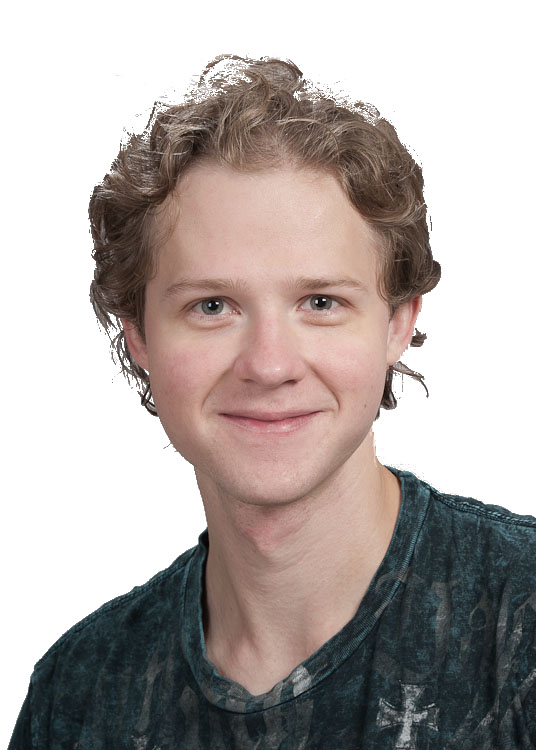
\includegraphics[width=1in,height=1.25in,clip,keepaspectratio]{photos/medley.jpg}}]{J. Kyle Medley}
is currently pursuing a Ph.D. in Bioengineering from the University of Washington, USA.
His research interests include modeling dynamical biophysical processes such as
metabolism and gene expression regulation.
He currently develops libRoadRunner, a software package used to simulate dynamical models encoded in SBML.
\end{IEEEbiography}

\begin{IEEEbiography}[{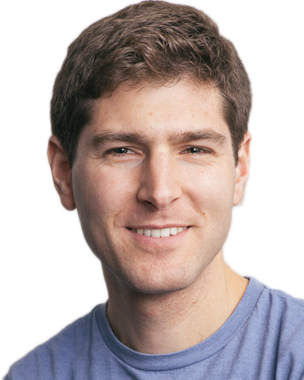
\includegraphics[width=1in,height=1.25in,clip,keepaspectratio]{photos/karr.jpg}}]{Jonathan R. Karr}
received his Ph.D. in Biophysics and M.S. in Medicine from Stanford University, USA in 2014 and his B.S.s in Physics and Brain \& Cognitive Sciences from the Massachusetts Institute of Technology, USA in 2006. Currently, Dr. Karr is a Fellow at the Icahn School of Medicine at Mount Sinai, USA. His research focuses on the development of comprehensive whole-cell computational models and their applications to bioengineering and medicine.
\end{IEEEbiography}

\vfill

\end{document}